% !TeX program = xelatex
% 自编练习，参照 2025 年秋季 A/B 卷结构。独立 XeLaTeX 源文件。
\documentclass[UTF8,11pt,a4paper,fontset=fandol]{ctexart}
\usepackage[top=18mm,bottom=18mm,left=21mm,right=21mm,footskip=9mm]{geometry}
\usepackage{amsmath,amssymb,array,tabularx,enumitem,fancyhdr,tikz}
\usetikzlibrary{arrows.meta}
\setlength{\parindent}{0pt}
\setlength{\parskip}{0.3em}
\linespread{1.12}\selectfont
\setlength{\headheight}{14pt}
\pagestyle{fancy}\fancyhf{}
\fancyfoot[C]{\small\thepage}
\renewcommand{\headrulewidth}{0pt}
\newcolumntype{Y}{>{\centering\arraybackslash}X}
\newcommand{\sect}[1]{\par\vspace{0.7em}{\large\bfseries #1}\par\vspace{0.6em}}
\newcommand{\choices}[4]{\par\nopagebreak\begin{tabularx}{\linewidth}{@{}XX@{}}A．#1&B．#2\\C．#3&D．#4\end{tabularx}\par}
\newcommand{\verticalchoices}[4]{\par\nopagebreak A．#1\par B．#2\par C．#3\par D．#4\par}
\newcommand{\ans}[1]{\par\textbf{解析：}#1\par}
\begin{document}
\fancyhead[R]{\small 宏观经济学期中模拟卷 · 参考答案与评分细则}
{\Large\bfseries 模拟卷一参考答案}\par
\smallskip 每卷满分 88 分。各题采用课件的简化模型；合理的等价推导和规范图形均可得分。
\sect{一、判断题（每题 2 分，共 20 分）}
\par\smallskip\begin{tabularx}{\linewidth}{|*{10}{Y|}}\hline
1&2&3&4&5&6&7&8&9&10\\\hline
$\surd$&$\surd$&$\times$&$\times$&$\times$&$\surd$&$\times$&$\surd$&$\times$&$\surd$\\\hline
\end{tabularx}\par\smallskip
\begin{enumerate}[label=\arabic*.,leftmargin=*,itemsep=0.7em,topsep=0.3em]
\item 企业当期在境内生产、但年末尚未售出的最终产品，应作为当期存货投资计入 GDP。
\ans{当期生产已经发生，未售出部分形成存货投资。是否售出不改变它属于当期产出的事实。}
\item 居民购买一件进口消费品时，消费和进口可以同时增加；在不考虑国内销售服务的情况下，这笔购买不直接增加本国 GDP。
\ans{进口品计入消费，同时通过净出口中的进口项扣除，二者相抵。国内提供的销售服务应另行核算。}
\item 若 CPI 和 GDP 平减指数在同一基年都等于 100，则此后两种指数的年度涨幅必然相同。
\ans{共同基年只确定指数尺度。CPI 与平减指数的商品范围及数量权重不同，后续变动可以不同。}
\item 在技术和其他投入不变时，资本边际收益递减意味着资本存量增加会使总产出下降。
\ans{边际收益递减指新增一单位资本带来的产出增量变小；边际产出仍为正时，总产出仍然增加。}
\item 在教材生产函数 $Y=AF(L,K,H,N)$ 中，$N$ 表示人口数量。
\ans{$N$ 表示自然资源；$L$ 是劳动，$K$ 是物质资本，$H$ 是人力资本，$A$ 是技术知识。}
\item 一个封闭经济体即使存在政府预算赤字，其国民储蓄仍然可能为正。
\ans{国民储蓄等于私人储蓄与公共储蓄之和。私人储蓄大于预算赤字时，二者之和仍为正。}
\item 在竞争性劳动市场的简单模型中，只要存在法定最低工资，无论其水平高低，都会造成结构性失业。
\ans{最低工资必须高于市场均衡工资、形成约束，才会在该模型中造成劳动供给超过劳动需求。}
\item 效率工资理论认为，企业有时会主动支付高于市场均衡水平的工资，以减少人员流失或提高工作努力程度。
\ans{较高工资可能降低离职率、提高努力程度和应聘者质量；这些收益可能使企业愿意主动支付较高工资。}
\item 在公众不持有现金的简单银行体系中，若法定准备金率为 20\%，而所有银行的实际准备金率均为 25\%，则货币乘数为 5。
\ans{应使用实际准备金率：$m=1/0.25=4$，不能用法定比率替代包含超额准备金的实际比率。}
\item 若货币流通速度与实际产出均不变，货币数量增加 8\%，价格水平也增加 8\%。
\ans{由 $P=MV/Y$，在 $V,Y$ 不变时，$P$ 与 $M$ 同比例变化。这里明确给出了必要条件。}
\end{enumerate}
\newpage\sect{二、单选题（每题 4 分，共 28 分）}
\par\smallskip\begin{tabularx}{\linewidth}{|*{7}{Y|}}\hline
1&2&3&4&5&6&7\\\hline
B&A&C&D&B&C&A\\\hline
\end{tabularx}\par\smallskip
\begin{enumerate}[label=\arabic*.,start=1,leftmargin=*,itemsep=1.05em]
\item 小林以 80 万元购买一套五年前建成的旧住房，并另外支付当期房产中介服务费 2 万元。忽略其他交易，这两笔支出合计对本期 GDP 的直接贡献为多少万元？
\choices{0}{2}{80}{82}
\ans{\textbf{B。}旧房本体是过去的产出，不重复计入当期 GDP；当期中介服务新创造了 2 万元服务产出。}
\item 某封闭经济体当年 $Y=1800$、$C=1100$、$G=400$、净税收 $T=350$。国民储蓄和投资分别为多少？
\choices{300 和 300}{350 和 350}{300 和 350}{350 和 300}
\ans{\textbf{A。}$S=Y-C-G=300$，封闭经济中 $I=S=300$。私人储蓄为 350，公共储蓄为 $-50$，不能把私人储蓄直接当成国民储蓄。}
\item 本国生产的一种工业设备全部出口，不进入本国居民消费篮子。当期只有该设备价格上涨，所有商品产量及其他价格均不变。其直接影响是：
\choices{CPI 上升，GDP 平减指数不变}{CPI 与 GDP 平减指数都上升}{CPI 不变，GDP 平减指数上升}{两个指数都不变}
\ans{\textbf{C。}出口设备属于本国当期产出，进入 GDP 平减指数；它不属于本国居民消费篮子，不直接进入 CPI。}
\item 某国名义 GDP 从 800 增至 924，GDP 平减指数从 100 增至 110。该国实际 GDP 增长率为：
\choices{10\%}{15.5\%}{4.5\%}{5\%}
\ans{\textbf{D。}实际 GDP 从 $800/(100/100)=800$ 增至 $924/(110/100)=840$，增长率为 $840/800-1=5\%$。不能直接用名义增长率减物价涨幅作为精确值。}
\end{enumerate}
\newpage\sect{二、单选题解析（续）}
\begin{enumerate}[label=\arabic*.,start=5,leftmargin=*,itemsep=1.05em]
\item 一家企业组织员工学习使用已有的生产软件，社会掌握的生产方法并未因此改变。这主要增加了生产函数中的哪一项？
\choices{物质资本 $K$}{人力资本 $H$}{自然资源 $N$}{技术知识 $A$}
\ans{\textbf{B。}培训提高劳动者掌握和应用现有知识的能力，属于人力资本积累；它与社会发现新的生产方法不同。}
\item 假设劳动力总量不变，每期就业者失去工作的比例为 $s=2\%$，失业者找到工作的比例为 $f=18\%$。稳态失业率为：
\choices{2\%}{9\%}{10\%}{20\%}
\ans{\textbf{C。}稳态满足 $sE=fU$，所以 $u=s/(s+f)=0.02/(0.02+0.18)=10\%$。分母不是单独的求职成功率。}
\item 初始货币数量 $M=400$、流通速度 $V=5$、实际产出 $Y=1000$。之后 $M$ 增至 440，$Y$ 增至 1100，$V$ 不变。价格水平将：
\choices{保持不变}{上升 $10\%$}{下降 $10\%$}{上升 $21\%$}
\ans{\textbf{A。}初始 $P=400\times5/1000=2$，之后 $P=440\times5/1100=2$。货币与实际产出同比增长，物价不变。}
\end{enumerate}
\medskip\textbf{核对提醒：}
实际 GDP 与价格指数要使用相同基年；稳态失业率的分母为 $s+f$；数量方程中的比例结论取决于 $V$ 和 $Y$ 的条件。
\newpage\sect{三、计算题（20 分）}
某经济体共有 200 名成年人。初始失业率为 12\%，劳动参与率为 75\%。所有人数均为实际人数，无须作整数近似。

\textbf{说明：}情景 I 与情景 II 相互独立，均从初始状态出发；成年人口总数始终不变。百分比保留两位小数即可。

\textbf{（1）计算初始的劳动力、就业人口、失业人口和非劳动力人口。（6 分）}
\ans{劳动力为 $200\times75\%=150$ 人；失业人口为 $150\times12\%=18$ 人；就业人口为 $150-18=132$ 人；非劳动力人口为 $200-150=50$ 人。劳动力与非劳动力合计 2 分，失业人口 2 分，就业人口 2 分。}

\textbf{（2）情景 I：12 名初始就业者失去工作，并继续积极求职；另外，15 名初始失业者停止求职并退出劳动力市场。其他人状态不变。计算新的失业率和劳动参与率。（6 分）}
\ans{12 名就业者转为失业者，15 名原失业者转为非劳动力，故 $E_1=132-12=120$，$U_1=18+12-15=15$，$L_1=135$，非劳动力为 65 人。失业率为 $15/135\times100\%\approx11.11\%$；劳动参与率为 $135/200\times100\%=67.50\%$。正确更新就业与失业人数各 1 分，两项比率各 2 分。}

\textbf{（3）情景 II：30 名初始非劳动力重新进入劳动力市场，其中 12 人立即找到工作，另外 18 人积极求职但尚未找到工作。其他人状态不变。计算新的失业率和劳动参与率。（6 分）}
\ans{劳动力增至 $L_2=150+30=180$，就业增至 $E_2=132+12=144$，失业增至 $U_2=18+18=36$，非劳动力为 20 人。失业率为 $36/180\times100\%=20.00\%$；劳动参与率为 $180/200\times100\%=90.00\%$。正确更新劳动力与失业人数各 1 分，两项比率各 2 分。}

\textbf{（4）分别将情景 I、II 与初始状态比较，说明为什么不能仅凭失业率升降判断就业状况是否改善。（2 分）}
\ans{情景 I 中失业率由 12\% 降至 11.11\%，但就业人数由 132 降至 120；失业者退出使分子、分母同时缩小。情景 II 中失业率升至 20\%，但就业人数升至 144；新进入者中有较多人仍在求职。指出任一比率与就业变化的背离并说明原因得 1 分，两种情景均解释正确共 2 分。}
\newpage\sect{四、作图分析题（20 分）}
请使用封闭经济的可贷资金市场模型，分析下列三个相互独立的情景。横轴为可贷资金数量，纵轴为实际利率 $r$；国民储蓄供给曲线向右上倾斜，投资需求曲线向右下倾斜。除题目明确给出的变化外，其他条件不变，产出 $Y$ 固定。每问均须作图，标出新旧曲线、均衡点，并解释均衡利率与投资数量的变化。
\begin{center}
\begin{minipage}[t]{0.33\linewidth}\centering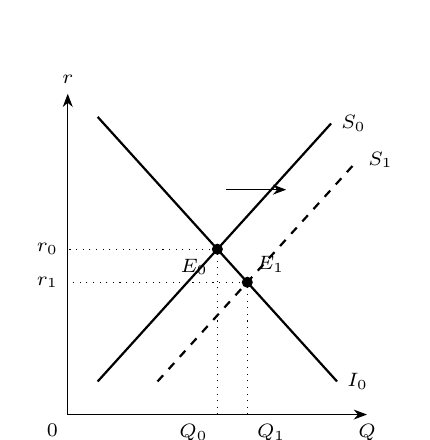
\begin{tikzpicture}[x=0.38cm,y=0.42cm,>=Stealth,font=\scriptsize]
\draw[->] (0,0)--(10,0) node[below] {$Q$};
\draw[->] (0,0)--(0,9.7) node[above] {$r$};
\node[below left] at (0,0) {$0$};
\draw[thick] (1,1)--(8.8,8.8) node[right] {$S_0$};
\draw[thick] (1,9)--(9,1) node[right] {$I_0$};
\draw[thick,dashed] (3,1)--(9.7,7.7) node[right] {$S_1$};\draw[->] (5.3,6.8)--(7.3,6.8);\draw[dotted] (5,0)--(5,5)--(0,5);\fill (5,5) circle(2pt) node[below left] {$E_0$};
\node[left] at (0,5) {$r_0$};
\node[below left] at (5,0) {$Q_0$};
\draw[dotted] (6,0)--(6,4)--(0,4);\fill (6,4) circle(2pt) node[above right] {$E_1$};
\node[left] at (0,4) {$r_1$};
\node[below right] at (6,0) {$Q_1$};
\end{tikzpicture}\par（1）\end{minipage}\hfill%
\begin{minipage}[t]{0.33\linewidth}\centering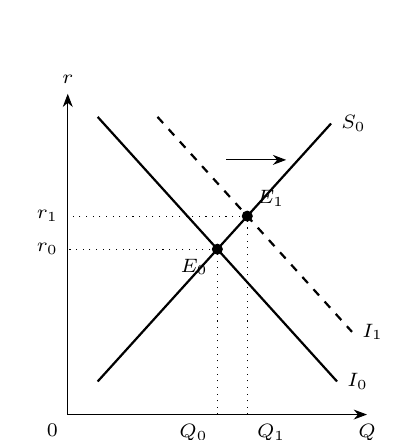
\begin{tikzpicture}[x=0.38cm,y=0.42cm,>=Stealth,font=\scriptsize]
\draw[->] (0,0)--(10,0) node[below] {$Q$};
\draw[->] (0,0)--(0,9.7) node[above] {$r$};
\node[below left] at (0,0) {$0$};
\draw[thick] (1,1)--(8.8,8.8) node[right] {$S_0$};
\draw[thick] (1,9)--(9,1) node[right] {$I_0$};
\draw[thick,dashed] (3,9)--(9.5,2.5) node[right] {$I_1$};\draw[->] (5.3,7.7)--(7.3,7.7);\draw[dotted] (5,0)--(5,5)--(0,5);\fill (5,5) circle(2pt) node[below left] {$E_0$};
\node[left] at (0,5) {$r_0$};
\node[below left] at (5,0) {$Q_0$};
\draw[dotted] (6,0)--(6,6)--(0,6);\fill (6,6) circle(2pt) node[above right] {$E_1$};
\node[left] at (0,6) {$r_1$};
\node[below right] at (6,0) {$Q_1$};
\end{tikzpicture}\par（2）\end{minipage}\hfill%
\begin{minipage}[t]{0.33\linewidth}\centering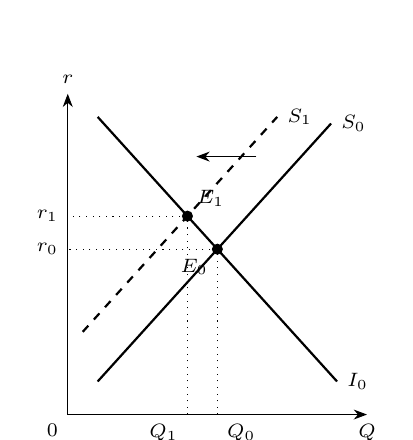
\begin{tikzpicture}[x=0.38cm,y=0.42cm,>=Stealth,font=\scriptsize]
\draw[->] (0,0)--(10,0) node[below] {$Q$};
\draw[->] (0,0)--(0,9.7) node[above] {$r$};
\node[below left] at (0,0) {$0$};
\draw[thick] (1,1)--(8.8,8.8) node[right] {$S_0$};
\draw[thick] (1,9)--(9,1) node[right] {$I_0$};
\draw[thick,dashed] (0.5,2.5)--(7,9) node[right] {$S_1$};\draw[->] (6.3,7.8)--(4.3,7.8);\draw[dotted] (5,0)--(5,5)--(0,5);\fill (5,5) circle(2pt) node[below left] {$E_0$};
\node[left] at (0,5) {$r_0$};
\node[below right] at (5,0) {$Q_0$};
\draw[dotted] (4,0)--(4,6)--(0,6);\fill (4,6) circle(2pt) node[above right] {$E_1$};
\node[left] at (0,6) {$r_1$};
\node[below left] at (4,0) {$Q_1$};
\end{tikzpicture}\par（3）\end{minipage}\hfill%
\end{center}
{\small 图中实线表示初始曲线，虚线表示变动后的曲线；$E_0,E_1$ 为初始与新均衡。图形仅示意方向，不表示题目数据的比例。}

\textbf{（1）政府削减政府购买，净税收不变；在每一个给定利率下，私人储蓄均不变。（6 分）}
\ans{给定利率下，$S_{\text{私人}}=Y-T-C$ 不变，$S_{\text{公共}}=T-G$ 增加，因此国民储蓄增加（2 分）。供给曲线从 $S_0$ 右移至 $S_1$，投资需求曲线不变（1 分）；均衡实际利率下降，投资增加（1 分）；坐标轴、曲线方向及新旧均衡正确（2 分）。}

\textbf{（2）技术革新提高了新建厂房与设备的预期回报，使每一个给定利率下的投资需求增加；储蓄供给行为不变。（6 分）}
\ans{项目回报提高使各利率下投资意愿增加，投资需求曲线从 $I_0$ 右移至 $I_1$（机制 2 分、位移 1 分）。储蓄供给曲线不变，均衡利率上升、均衡投资增加（1 分）。储蓄量增加表现为沿供给曲线移动。图形完整正确（2 分）。}

\textbf{（3）净税收增加 100，政府购买增加 80；在每一个给定利率下，居民消费因增税减少 60。投资需求曲线不变。请先分别计算私人储蓄、公共储蓄与国民储蓄的变化，再作图分析。（8 分）}
\ans{在给定利率下，私人储蓄变化为 $\Delta S_{\text{私人}}=-\Delta T-\Delta C=-100-(-60)=-40$（2 分）；公共储蓄变化为 $\Delta S_{\text{公共}}=100-80=20$（2 分）；国民储蓄变化为 $-40+20=-20$（1 分）。供给曲线左移，投资需求曲线不变（1 分），均衡利率上升、投资下降（1 分），图形正确（1 分）。公共储蓄改善并不保证国民储蓄增加；20 是给定利率下的供给位移量，不必等于新均衡投资的减少量。}
\newpage
{\Large\bfseries 模拟卷二参考答案}\par
\smallskip 每卷满分 88 分。各题采用课件的简化模型；合理的等价推导和规范图形均可得分。
\sect{一、判断题（每题 2 分，共 20 分）}
\par\smallskip\begin{tabularx}{\linewidth}{|*{10}{Y|}}\hline
1&2&3&4&5&6&7&8&9&10\\\hline
$\surd$&$\times$&$\surd$&$\surd$&$\times$&$\times$&$\surd$&$\times$&$\surd$&$\times$\\\hline
\end{tabularx}\par\smallskip
\begin{enumerate}[label=\arabic*.,leftmargin=*,itemsep=0.7em,topsep=0.3em]
\item 政府发放养老金属于转移支付，养老金本身不计入 GDP 支出法中的政府购买。
\ans{转移支付不对应政府购买当期物品或服务。领取者后来购买的当期产品另按相应支出项目核算。}
\item 只要两国人均实际 GDP 相同，就可以断定两国居民的经济福利水平相同。
\ans{人均 GDP 未充分反映收入分配、闲暇、环境质量和非市场劳动等，因此不能保证福利相同。}
\item 固定消费篮子没有及时反映消费者转向相对便宜商品的行为，可能高估生活费用的上升。
\ans{这就是替代偏向：价格变化后消费者可以调整购买组合，固定篮子不能充分体现这种调整。}
\item 生产函数具有规模报酬不变，与资本的边际收益递减可以同时成立。
\ans{前者考察全部投入同比例变化，后者固定其他投入、只增加资本，两者考察的变化不同。}
\item 在技术不进步、其他相关条件不变的资本积累模型中，一次性提高储蓄率必然使人均实际产出的增长率永久提高。
\ans{较高储蓄率可以加快过渡期增长、提高长期人均产出水平；递减收益使它不能单独维持永久更高的增长率。}
\item 公司发行债券和发行股票都使购买者成为公司的部分所有者，并享有相同的剩余利润索取权。
\ans{债券持有人是债权人，股票持有人才是部分所有者；二者的收益约定和索取权不同。}
\item 在劳动力总量不变的两状态模型中，若失去工作的概率不变，而失业者找到工作的概率上升，则稳态失业率下降。
\ans{稳态失业率 $u=s/(s+f)$；固定 $s$，提高 $f$ 会降低 $u$。}
\item 在成年人口总数不变时，统计失业率下降必然意味着就业人数增加。
\ans{失业者停止求职会同时减少失业人数和劳动力人数，即使就业人数不变，失业率也可能下降。}
\item 居民把原来持有的纸币存入活期账户，在银行尚未据此发放新贷款的瞬间，流通中现金减少与活期存款增加相抵，货币总量不变。
\ans{按现金加活期存款的简单货币口径，这一瞬间只是货币形式转换。银行后续贷款可能进一步创造存款。}
\item 仅凭数量方程 $MV=PY$，无须对 $V$ 和 $Y$ 作任何假设，就能推出货币数量增长 10\% 必使价格水平增长 10\%。
\ans{$V$ 或 $Y$ 也可能变化。只有在二者均不变等明确条件下，才能推出 $P$ 与 $M$ 同比例变化。}
\end{enumerate}
\newpage\sect{二、单选题（每题 4 分，共 28 分）}
\par\smallskip\begin{tabularx}{\linewidth}{|*{7}{Y|}}\hline
1&2&3&4&5&6&7\\\hline
B&C&A&D&C&B&D\\\hline
\end{tabularx}\par\smallskip
\begin{enumerate}[label=\arabic*.,start=1,leftmargin=*,itemsep=1.05em]
\item 小周存入银行 1 万元，一年名义利率为 6\%。同期 CPI 从 120 上升到 127.2。忽略税费，小周一年后本息的购买力相对于存款时：
\choices{提高}{不变}{降低}{无法判断}
\ans{\textbf{B。}通胀率为 $127.2/120-1=6\%$；实际收益率为 $1.06/1.06-1=0$，购买力不变。这是实际利率计算，不涉及费雪效应。}
\item 某消费篮子固定包含 2 份食品和 3 次公交出行。基年食品单价为 5 元、公交单价为 2 元；本年分别为 6 元、4 元。以基年 CPI 为 100，本年 CPI 为：
\choices{125}{140}{150}{160}
\ans{\textbf{C。}基年篮子费用 $2\times5+3\times2=16$ 元，本年费用 $2\times6+3\times4=24$ 元，故 CPI 为 $24/16\times100=150$。应固定数量，而非对两个价格涨幅作简单平均。}
\item 封闭经济体中，$Y=2000$、$C=1250$、$G=450$、净税收 $T=300$。私人储蓄、公共储蓄和国民储蓄依次为：
\choices{$450,\;-150,\;300$}{$300,\;-150,\;150$}{$450,\;150,\;600$}{$300,\;150,\;450$}
\ans{\textbf{A。}私人储蓄为 $2000-300-1250=450$；公共储蓄为 $300-450=-150$；国民储蓄为 $450-150=300$。}
\item 某经济体实际 GDP 一年增长 8.12\%，同期人口增长 2\%。按精确公式计算，人均实际 GDP 增长率为：
\choices{8.12\%}{6.12\%}{4.06\%}{6\%}
\ans{\textbf{D。}人均实际 GDP 增长率为 $1.0812/1.02-1=6\%$。总量除以人口，因此增长因子相除，而非简单相减。}
\end{enumerate}
\newpage\sect{二、单选题解析（续）}
\begin{enumerate}[label=\arabic*.,start=5,leftmargin=*,itemsep=1.05em]
\item 以下哪种情况最符合摩擦性失业的含义？
\choices{约束性最低工资使部分求职者无法就业}{总需求下降导致企业裁员}{毕业生花时间寻找更匹配自身能力的职位}{产业转型后劳动者技能与现有岗位长期不匹配}
\ans{\textbf{C。}寻找合适岗位需要时间，属于摩擦性失业；最低工资约束和持续技能不匹配偏向结构性失业，经济衰退导致的裁员偏向周期性失业。}
\item 在公众不持有现金、所有银行实际准备金率保持 20\% 的简单模型中，央行向商业银行出售 20 亿元政府债券，银行以准备金支付。假定体系完成存款收缩且其他条件不变，货币供给最终变化为：
\choices{增加 100 亿元}{减少 100 亿元}{减少 20 亿元}{增加 20 亿元}
\ans{\textbf{B。}准备金减少 20 亿元，货币乘数为 $1/0.20=5$，故最终货币供给变化为 $-20\times5=-100$ 亿元。需要题设给定的调整完成与实际准备金率不变。}
\item 某经济体 $M=600$、$V=4$、实际 GDP 为 1500。若数量方程中的 $P$ 以基期为 1，而 GDP 平减指数以基期为 100，则该平减指数为：
\choices{120}{150}{180}{160}
\ans{\textbf{D。}$P=MV/Y=600\times4/1500=1.6$，换成基期为 100 的指数后为 160。不能把价格倍数 1.6 与指数数值 160 混用。}
\end{enumerate}
\medskip\textbf{核对提醒：}
实际利率按购买力变化计算；公开市场操作题须区分准备金变化和最终货币变化；基期为 100 的价格指数须除以 100 后才能作为 $P$ 代入数量方程。
\newpage\sect{三、计算题（20 分）}
某商业银行初始资产负债表如下，单位均为亿元。存款为公众的活期存款，一般性债务不计入本题的货币总量。
\begin{center}\renewcommand{\arraystretch}{1.35}
\begin{tabularx}{0.9\linewidth}{|X|r|X|r|}\hline
\multicolumn{2}{|c|}{资产}&\multicolumn{2}{c|}{负债和所有者权益}\\\hline
存款准备金&80&存款&400\\\hline
贷款&300&一般性债务&50\\\hline
有价证券&120&资本（所有者权益）&50\\\hline
合计&500&合计&500\\\hline
\end{tabularx}\end{center}

\textbf{说明：}两个情景相互独立，均从初始资产负债表出发。杠杆率定义为资产总额除以所有者权益；账面所有者权益允许为负，须与股东本金的损失比例区分。

\textbf{（1）计算该银行的实际存款准备金率和杠杆率。若所有银行均保持这一实际准备金率，公众不持有现金，计算简单模型中的货币乘数。（6 分）}
\ans{初始资产总额为 $80+300+120=500$，负债为 $400+50=450$，权益为 50。实际准备金率为 $80/400=20\%$（2 分）；杠杆率为 $500/50=10$ 倍（2 分）；货币乘数为 $1/0.20=5$（2 分）。杠杆率分母是权益，准备金率分母是存款，二者不能混用。}

\textbf{（2）情景 I：股东向银行追加资本 50 亿元，这笔资金全部计入该银行准备金；存款、一般性债务及其他资产项目均不变。计算新的资产总额、所有者权益和杠杆率，并判断银行在权益耗尽前可吸收的资产损失比例是上升还是下降。（7 分）}
\ans{追加资本后，准备金为 $80+50=130$，资产总额为 $550$（2 分）；存款与一般债务仍合计 450，所以权益为 $550-450=100$（2 分）。杠杆率为 $550/100=5.5$ 倍（2 分）。权益占资产比重由 $50/500=10\%$ 升至 $100/550\approx18.18\%$，故可吸收的资产损失比例上升（方向正确 1 分）。追加资本不同于新增负债。}

\textbf{（3）情景 II：初始贷款资产发生 20\% 的损失，其他资产和全部负债不变，且无人追加资本。计算账面所有者权益及其相对初始权益的变化百分比；另在股东有限责任且不再出资的条件下，指出原股东本金的损失比例。（7 分）}
\ans{贷款损失为 $300\times20\%=60$（2 分），资产总额降至 $500-60=440$，负债仍为 450，账面权益为 $440-450=-10$（2 分）。账面权益变化百分比为 $(-10-50)/50\times100\%=-120\%$（2 分），银行已资不抵债。原股东本金全部损失，有限责任下本金损失比例为 100\%（1 分）。负账面权益 10 亿元不是原股东必须继续支付的本金损失。}
\newpage\sect{四、作图分析题（20 分）}
请采用课件中的长期货币供求模型，分别分析下列三个相互独立的情景。横轴为名义货币量 $M$，纵轴为货币价值 $1/P$；货币供给曲线垂直，货币需求曲线向右下倾斜。除题目明确给出的变化外，其他条件不变。每问均须标出新旧曲线、均衡点，并解释均衡名义货币量与价格水平的变化。
\begin{center}
\begin{minipage}[t]{0.33\linewidth}\centering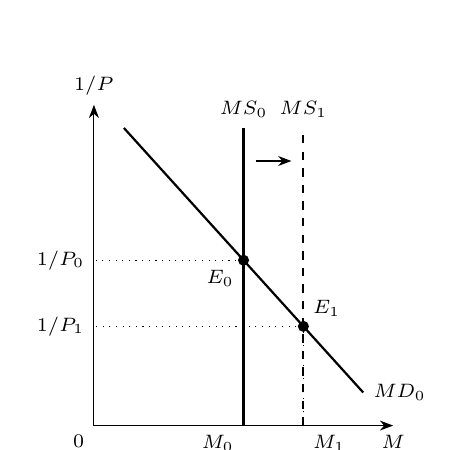
\begin{tikzpicture}[x=0.38cm,y=0.42cm,>=Stealth,font=\scriptsize]
\draw[->] (0,0)--(10,0) node[below] {$M$};
\draw[->] (0,0)--(0,9.7) node[above] {$1/P$};
\node[below left] at (0,0) {$0$};
\draw[thick] (5,0)--(5,9) node[above] {$MS_0$};\draw[thick] (1,9)--(9,1) node[right] {$MD_0$};\draw[thick,dashed] (7,0)--(7,9) node[above] {$MS_1$};\draw[->] (5.4,8)--(6.6,8);\draw[dotted] (5,0)--(5,5)--(0,5);\fill (5,5) circle(2pt) node[below left] {$E_0$};
\node[left] at (0,5) {$1/P_0$};
\node[below left] at (5,0) {$M_0$};
\draw[dotted] (7,0)--(7,3)--(0,3);\fill (7,3) circle(2pt) node[above right] {$E_1$};
\node[left] at (0,3) {$1/P_1$};
\node[below right] at (7,0) {$M_1$};
\end{tikzpicture}\par（1）\end{minipage}\hfill%
\begin{minipage}[t]{0.33\linewidth}\centering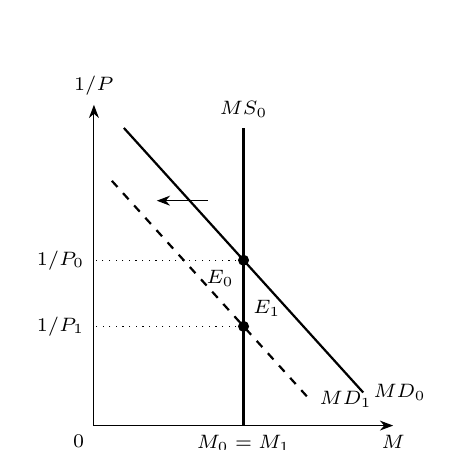
\begin{tikzpicture}[x=0.38cm,y=0.42cm,>=Stealth,font=\scriptsize]
\draw[->] (0,0)--(10,0) node[below] {$M$};
\draw[->] (0,0)--(0,9.7) node[above] {$1/P$};
\node[below left] at (0,0) {$0$};
\draw[thick] (5,0)--(5,9) node[above] {$MS_0$};\draw[thick] (1,9)--(9,1) node[right] {$MD_0$};\draw[thick,dashed] (0.6,7.4)--(7.2,0.8) node[right] {$MD_1$};\draw[->] (3.8,6.8)--(2.1,6.8);\draw[dotted] (5,0)--(5,5)--(0,5);\fill (5,5) circle(2pt) node[below left] {$E_0$};
\node[left] at (0,5) {$1/P_0$};
\draw[dotted] (5,0)--(5,3)--(0,3);\fill (5,3) circle(2pt) node[above right] {$E_1$};
\node[left] at (0,3) {$1/P_1$};
\node[below] at (5,0) {$M_0=M_1$};
\end{tikzpicture}\par（2）\end{minipage}\hfill%
\begin{minipage}[t]{0.33\linewidth}\centering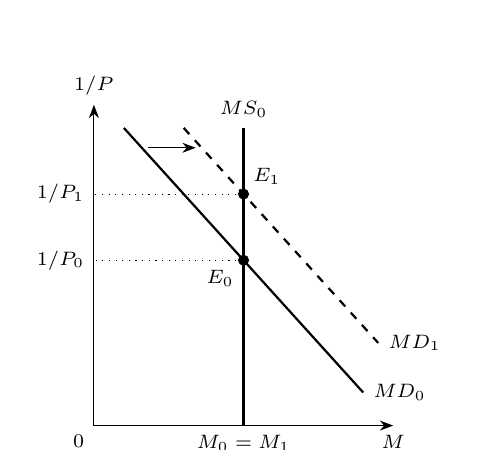
\begin{tikzpicture}[x=0.38cm,y=0.42cm,>=Stealth,font=\scriptsize]
\draw[->] (0,0)--(10,0) node[below] {$M$};
\draw[->] (0,0)--(0,9.7) node[above] {$1/P$};
\node[below left] at (0,0) {$0$};
\draw[thick] (5,0)--(5,9) node[above] {$MS_0$};\draw[thick] (1,9)--(9,1) node[right] {$MD_0$};\draw[thick,dashed] (3,9)--(9.5,2.5) node[right] {$MD_1$};\draw[->] (1.8,8.4)--(3.4,8.4);\draw[dotted] (5,0)--(5,5)--(0,5);\fill (5,5) circle(2pt) node[below left] {$E_0$};
\node[left] at (0,5) {$1/P_0$};
\draw[dotted] (5,0)--(5,7)--(0,7);\fill (5,7) circle(2pt) node[above right] {$E_1$};
\node[left] at (0,7) {$1/P_1$};
\node[below] at (5,0) {$M_0=M_1$};
\end{tikzpicture}\par（3）\end{minipage}\hfill%
\end{center}
{\small 图中实线表示初始曲线，虚线表示变动后的曲线；$E_0,E_1$ 为初始与新均衡。图形仅示意方向，不表示题目数据的比例。}

\textbf{（1）央行在公开市场买入政府债券，使银行体系准备金增加。实际准备金率及公众持币习惯不变，货币需求曲线不变。（6 分）}
\ans{央行买入债券增加准备金，在实际准备金率与持币习惯不变时，银行体系扩张存款，货币供给增加（2 分）。$MS_0$ 右移至 $MS_1$，$MD$ 不变（1 分）；新均衡名义货币量增加，$1/P$ 下降，价格水平 $P$ 上升（1 分）；坐标轴、曲线和新旧均衡正确（2 分）。}

\textbf{（2）一种新的支付方式使交易更加便利，在每一个给定物价水平下，人们希望持有的名义货币减少。货币供给保持不变。（6 分）}
\ans{支付便利性提高，使给定价格水平下所需交易余额减少（2 分），$MD_0$ 左移至 $MD_1$，垂直的货币供给曲线不动（1 分）。新均衡名义货币量不变，$1/P$ 下降，$P$ 上升（1 分）；图形正确（2 分）。这里通过价格调整恢复供求平衡。}

\textbf{（3）其他非货币资产的收益率下降，且这些资产的流动性与风险不变。货币供给保持不变。请进一步判断实际货币余额的变化，并解释为何货币需求曲线移动后，均衡名义货币量不一定改变。（8 分）}
\ans{其他资产收益率下降降低了持有货币的机会成本，给定物价下人们愿意持有更多货币（2 分）；$MD_0$ 右移至 $MD_1$，$MS$ 不变（2 分）。均衡名义货币量仍等于固定供给量（1 分），$1/P$ 上升，故 $P$ 下降（1 分）；$M$ 不变而 $P$ 下降，实际货币余额 $M/P$ 增加（1 分）。完整图形正确（1 分）。需求曲线的位移是给定价格下意愿改变；新均衡通过价格调整满足同一名义货币供给。}
\end{document}
